% Social Media Analytics 2022/23

%%%%%%%%%%%%%%%%%%%%%%%%%%%%%%%%%%%%%%%%%%%%%%%%%%%%%%

% OPTIONAL PACKAGES
\documentclass[12pt,journal,compsoc]{IEEEtran}
\usepackage{amsfonts}
\usepackage{caption}
\usepackage{multirow}
\usepackage[table,xcdraw]{xcolor}
\usepackage{booktabs}
\usepackage{tabularx}
\usepackage[hyphens]{url}
\usepackage{biblatex}
\usepackage{blindtext,graphicx}
\usepackage[absolute]{textpos}
\usepackage[italian]{babel}
\usepackage{float}
\usepackage{hyperref}
\addbibresource{ref.bib} %Import the bibliography file

%%%%%%%%%%%%%%%%%%%%%%%%%%%%%%%%%%%%%%%%%%%%%%%%%%%%%%

\begin{document}

\begin{textblock}{5}(1,0.5)
\noindent\small Digital Signal And Image Management - UniMib 2022/23
\end{textblock}

\title{Project\\
\vspace{2mm}\large{Digital Signal And Image Management}}
\author{Agazzi Ruben 844736}

\IEEEtitleabstractindextext{%
\begin{abstract}
This project is divided in three parts: audio classification were I tried to classify urban sounds into 10 different classes using machine learning algorithms, image classification where I tried to classify images belonging to 10 different classes like "Forest", "Building", etc... and content based image retrieval on food images from a dataset containing 10 different types of food.
\end{abstract}}

\maketitle
\IEEEpeerreviewmaketitle
\IEEEdisplaynontitleabstractindextext

\tableofcontents

%%%%%%%%%%%%%%%%%%%%%%%%%%%%%%%%%%%%%%%%%%%%%%%%%%%%%%

\section{Audio classification}
The first task of the audio consists in the classification of 1-d audio signals into 10 different classes. I solved this task by doing some preprocessing of the dataset, feature extraction and finally classification using the features with a machine learning algorithm.
\subsection{Dataset}
The dataset can be found on Kaggle, it is called "UrbanSound8K"\cite{dataset1} and consists in sounds recorded in an urban environment.\\
The dataset contains 10 different classes:
\begin{itemize}
	\item Air conditioner
	\item Car horn
	\item Children playing
	\item Dog bark
	\item Engine Idling
	\item Gun shot
	\item Jackhammer
	\item Siren
	\item Street music
\end{itemize}
The dataset contains 8732 labeled sounds, and all the sound have a duration that is less or equal to 4 seconds.

\subsection{Preprocessing}
After an initial exploratory analysis of the audio data I found out that some audio were mono channel and some were stereo audio. For the stereo audio I took the first channel in order to process the data in an equal way for all the entries of the dataset.
\subsection{Feature extraction}
For the phase of feature extraction I decided to extract the following features:
\begin{itemize}
	\item Energy: is defined as the sum of the squared values of the audio $E = \sum_{n=-\infty}^\infty |x(n)|^2$
	\item Zero Crossing Rate: is defined as the number that the signal switch from a positive to a negative value or vice versa, divided by the length of the signal
	\item Spectrogram: Is an intensity plot of the fourier transform magnitude. It can be seen as a visual(2-d) representation\cite{spectrogram}
	\item Mel Spectrogram: the Mel spectogram is the spectogram with its value scaled by the Mel scale. The Mel scale was introduced because humans do not easilly tell the difference in the same ways for all the heard frequencies.
	\item MFCC features: is a representation of the short-term power spectrum of a sound\cite{MFCC}.
\end{itemize}
Some features, like the Mel spectogram, change according to the duration of the audio, but we cannot have features with different sizes for the classification part, so I decided to take the first 1 second for the extraction of these features.

\subsection{Classification}
After extracting the features I proceeded to the classification task. In this case i trained a Support Vector Machine and a Multi Layer Perceptron in order to compare them.
\subsubsection{Support Vector Machines}
Support vector machines are a type of machine learning algorithms that tries to classify data by triyng to linearly separate them. Because, in most of the cases, data are not linearly separable, it first applies a transformation to the data, for example it adds some dimensions to the data, in order to make them more easily separable

For the training of the Support Vector Machine I used the python library sklearn, in particular the LinearSVC classifier. I also tried different configurations for the SVC parameters:
\begin{itemize}
	\item C parameter: Is a regularization parameter, and the strenght of the regularization is inversely proportianl to its value. In this case the best parameter found was 
\end{itemize}
After training the classifier I tried it in the test dataset in order to evaluate it's performance. The accuracy of the classifier was equal to 69\% and the following values abount precision, recall and f1 on the 10 classes:
\begin{table}[ht]
	\centering
	\begin{tabular}{c c c c }
		Class & Precision & Recall & F1  \\
		\hline
		0 & 0.91 &0.84  &0.88        \\
		1 & 1.00 &0.31  &0.47        \\
		2 & 0.69 &0.58  &0.63        \\
		3 & 0.30 &0.83  &0.44        \\ 
		4 & 0.84 &0.64  &0.73        \\
		5 & 0.93 &0.83  &0.87        \\
		6 & 1.00 &0.33  &0.50        \\
		7 & 0.96 &0.85  &0.90        \\
		8 & 0.94 &0.67  &0.78        \\
		9 & 0.58 &0.54  &0.56        \\
	\end{tabular}
	\caption{Table of Precision, Recall and F1 measure on every class computed on the test dataset}
	\end{table}
	\begin{figure}[H]
		\begin{center}
		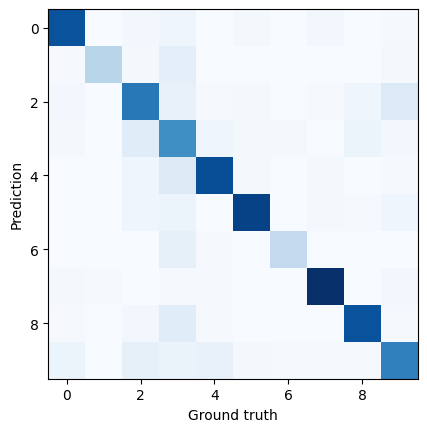
\includegraphics[scale=.75]{./images/confmat_soundClassification.png}
		\end{center}
		\caption{Confusion matrix of the classifier over the test dataset}
	\end{figure}

\subsubsection{Convolutional Neural Network}
The convolutional neural network composed by 11 layers. I also applied L2 regularization to the layers in order to prevent overfitting. The layers are the following:
\begin{itemize}
	\item First convolutional layer: Convolutional layer with 128 filters of size 3x3 with ReLU activation
	\item First max pooling layer: max pooling layer with window size of 2x2
	\item First flatten layer: flatten layer in order to pass the features to the dense layers
	\item First dense layer: Dense layer with 1024 neurons with ReLU activation
	\item Second dense layer: Dense layer with 512 neurons with ReLU activation
	\item Thirs dense layer: Dense layer with 256 neurons with ReLU activation
	\item Fourth dense layer: Dense layer with 128 neurons with ReLU activation
	\item First dropout: Dropout layer with probability of dropout of 0.2 to add regularization
	\item Fifth dense layer: Dense layer with 64 neurons with ReLU activation
	\item Second dropout: Dropout layer with probability of dropout of 0.1 to add regularization
	\item Output layer: Dense layer with 10 neurons with softmax activation to perform classification
\end{itemize}

The model reached an accuracy of 59.8\% on the validation set and an accuracy of 60\% on the test dataset. The model obtrained the followed precision, recall and F1 measure over the 10 classes: 
\begin{table}[ht]
	\centering
	\begin{tabular}{c c c c }
		Class & Precision & Recall & F1  \\
		\hline
		0 & 0.88 &0.52  &0.65     \\
		1 & 0.85 &0.67  &0.75      \\
		2 & 0.66 &0.31  &0.42       \\
		3 & 0.67 &0.58  &0.62        \\ 
		4 & 0.83 &0.66  &0.74        \\
		5 & 0.28 &0.91  &0.43        \\
		6 & 0.96 &0.70  &0.81       \\
		7 & 0.83 &0.64  &0.72        \\
		8 & 0.85 &0.61  &0.71        \\
		9 & 0.75 &0.45  &0.56        \\
	\end{tabular}
	\caption{Table of Precision, Recall and F1 measure on every class computed on the test dataset}
	\end{table}
	\begin{figure}[H]
		\begin{center}
		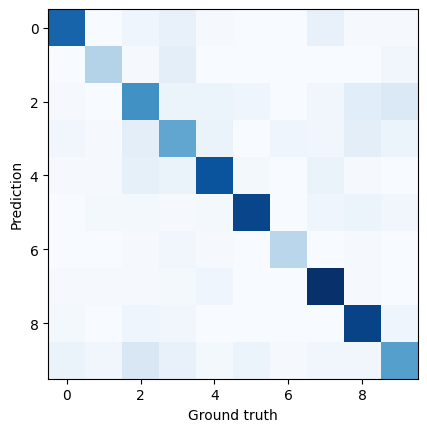
\includegraphics[scale=.75]{./images/confmat_sound_mlp.png}
		\end{center}
		\caption{Confusion matrix of the classifier over the test dataset}
	\end{figure}
\subsection{Evaluation}
The best performing model was the smv. This could be because for the convolutional neural network I only used MFCC features for classification. Maybe adding more features can lead to better result using this type of architecture. Also I observed making tests on downloaded data that both the models tends to predict always the same class, maybe there is some kind of overfitting over the dataset itself. This could be maybe fixed by using a larger dataset or by using better features for classification.
\section{Image classification}
For the image classification I tried to clasify images beloging to 6 different classes using a custom Convolutional Neural Network and using a pretrained Convolutional Neural Network.
\subsection{Dataset}
The dataset is the Intel Image Classification\cite{dataset2} available in Kaggle, it consists in 25000 rgb images of size 150x150 divided in 6 classes.
The classes are:
\begin{itemize}
	\item Buildings
	\item Glacier
	\item Mountain
	\item Sea 
	\item Street
\end{itemize}
\subsection{Convolutional Neural Networks}
Convolutional Neural Networrks are a class or artificial neural networks, most commonly used to analyze images\cite{CNNs}.
They are deep learning algorithms presenting convolutional layers: theese layers are composed by a fixed number of convolutional filters of a given dimension. The network during the training phase try to learn the weight of the components of the convolutional filters

\subsection{Custom CNN}
For the classification problem I designed a custom CNN that I later trained using the training data. The Network is composed by 14 layers:
\begin{itemize}
	\item Input layer: Input layer for images of size 150x150x3
	\item First Convolutional layer: Convolutional layer composed by 64 convolutional filters of size 3x3 with ReLU activation function.
	\item First average pooling: Average pooling layer with filter size 2x2
	\item Second Convolutional layer: Convolutional layer composed by 32 convolutional filters of size 3x3 with ReLU activation function.
	\item Second average pooling: Average pooling layer with filter size 2x2
	\item Third Convolutional layer: Convolutional layer composed by 16 convolutional filters of size 3x3 with ReLU activation function.
	\item Third average pooling: Average pooling layer with filter size 2x2
	\item First flatten layer: layer used to flatten the output of convolutional layers in order to have a vector of features to pass to the fully connected part of the network
	\item First dense layer: Dense layer with 512 neurons with ReLU activation function
	\item First dropout layer: Dropout layer with probability of 0.1 to prevent overfitting
	\item Second dense layer: Dense layer with 256 neurons with ReLU activation function
	\item Second dropout layer: Dropout layer with probability of 0.1 to prevent overfitting
	\item Third dense layer: Dense layer with 64 neurons with ReLU activation function
	\item Output layer: Dense layer with 6 neurons and softmax activation function in order to make the classification
\end{itemize}
The final network has a total of 2,539,894 trainable parameters.
I trained the network on the training dataset for 128 epochs obtaining an accuracy on the validation set equal to 76\% but an accurazy of 64\% on the test dataset.
\begin{table}[ht]
	\centering
	\begin{tabular}{c c c c }
		Class & Precision & Recall & F1  \\
		\hline
		0 & 0.65 &0.59 &0.62     \\
		1 & 0.81 &0.86 &0.83       \\
		2 & 0.57 &0.58 &0.58       \\
		3 & 0.54 &0.67 &0.60       \\ 
		4 & 0.57 &0.43 &0.49       \\
		5 & 0.73 &0.71 &0.72       \\
		
	\end{tabular}
	\caption{Table of Precision, Recall and F1 measure on every class computed on the test dataset}
	\end{table}
	\begin{figure}[H]
		\begin{center}
		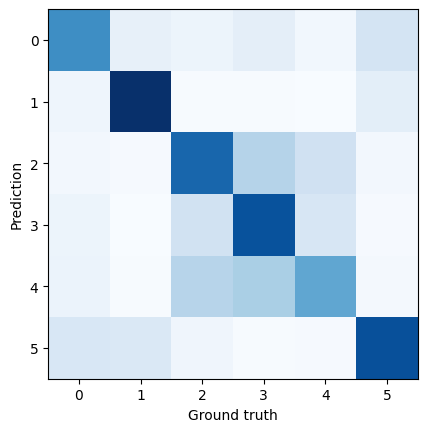
\includegraphics[scale=.75]{./images/confmat_cnn.png}
		\end{center}
		\caption{Confusion matrix of the classifier over the test dataset}
	\end{figure}
\subsection{Pretrained CNN}
In this other try i used a pretrained CNN, the VGG16\cite{VGG16} network using the ImageNet weights. I fine tuned the network in order to classify the data: I removed the initial input layer because the input size was greater than the dimension of the images of the dataset, and then I added 4 Dense layers at the end of the network that I trained to classify the images, in practice I use all the VGG16 network as a feature extractor. With this model I obtained an accuracy of 83.06\% on the validation dataset and of 81\% over the test set.
For the training of this model I also added a step of data augmentation in order to generate more images by sheering, rotating, zoomming and changing the brightness of the original images.
The classifier obtained the following metrics over the 6 classes:

\begin{table}[ht]
	\centering
	\begin{tabular}{c c c c }
		Class & Precision & Recall & F1  \\
		\hline
		0 & 0.85 & 0.92 &0.89     \\
		1 & 0.97 & 0.94 &0.95       \\
		2 & 0.68 &0.84  &0.75       \\
		3 & 0.88 &0.46  &0.60       \\ 
		4 & 0.69 &0.85  &0.76       \\
		5 & 0.89 & 0.88 &0.89       \\
		
	\end{tabular}
	\caption{Table of Precision, Recall and F1 measure on every class computed on the test dataset}
	\end{table}
	\begin{figure}[H]
		\begin{center}
		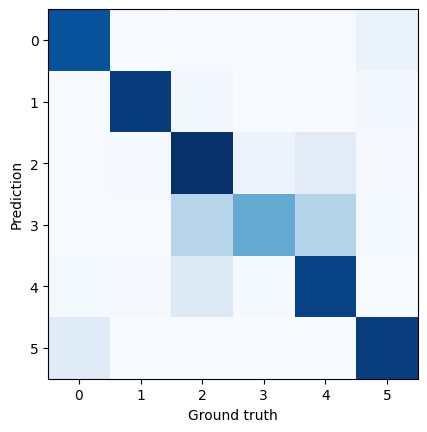
\includegraphics[scale=.75]{./images/confmat_vgg16.png}
		\end{center}
		\caption{Confusion matrix of the classifier over the test dataset}
	\end{figure}
\subsection{Evaluation}
After evaluating the two classifier the best one seems to be the fine tuned VGG16 model, because all the measures were higher than the convolutional neural network; but testing on some downloaded images from the internet, I saw that the fine tuned model always predicted the same class, while the other classifier predicted better classes for the images, even though it had problems like distinguishing a forest from a mountain if the forest had some altures, or distinguishing between a building and a street.

\section{Image retrieval}
For the part of image retrieval I used the same pretrained network used in the previous task, the VGG16 model. For this phase I made two tests: I used features for the retrieval coming from the third pooling layer and from the last pooling layer.
\subsection{Dataset}
The dataset is available on kaggle and is the "Fast Food Classification Dataset - V2"\cite{dataset3}. It contains 20.000 images belonging to 10 different classes:
\begin{itemize}
	\item Baked potato
	\item Burger
	\item Crispy Chicken
	\item Donut 
	\item Fries 
	\item Hot Dog 
	\item Pizza 
	\item Sandwich
	\item Taco 
	\item Taquito
\end{itemize}
\subsection{Feature extraction}
For the phase of feature extraction I used the pre-trained Concolutional Neural Network VGG16 and cutted the model at the third pooling layer. After extracting the feature i flatten them and finally save them in order to be used to find similar images. Teh final otained features have a dimansionality of 25088.
\begin{figure}[H]
  \begin{center}
  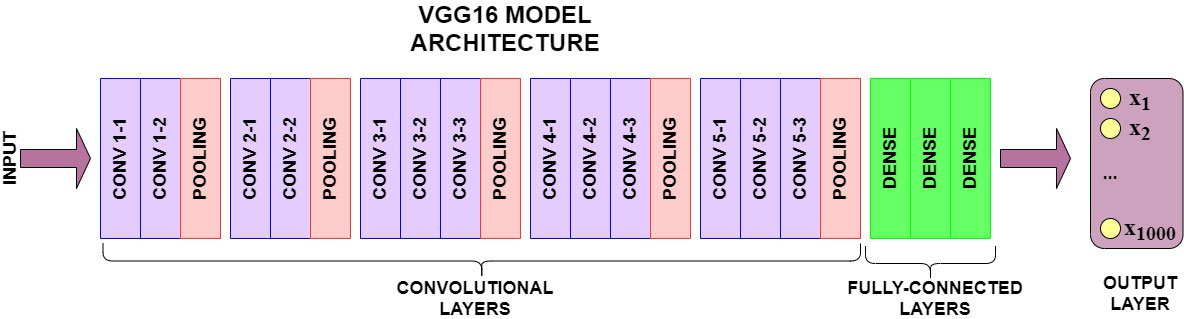
\includegraphics[scale=.20]{./images/vgg16-architecture.width-1200.jpg}
  \end{center}
  \caption{VGG16 model architecture}
\end{figure}
\subsection{Retrieval}
For the image retrieval task I used a k-d tree\cite{Kdtree}. A kd-tree is a structure, in particular a binary tree, used for storing a finite set of points form a k-dimensional space. It partitions the k-dimensional space in order to organize the points. This can lead to faster search performance of the point inside the k-dimensional space.
In this case I used the "pynanoflann"\cite{PyNanoflann} python lybrary, because was the only library I tried that could build the tree in reasonable time(a few seconds).
To retrieve the images starting from a test image we need to use the cutted VGG16 model to extract the features and then search for the most similar features inside the tree. The distance function used for searching the features inside the tree was the euclidean distance. The tree returns the 10 most similar features with the corresponding index.

\begin{figure}[H]
	 \[d(p, q) = \sqrt[]{(p_1-q_1)^2 +...+(p_n-q_n)^2} \]
	 \caption{Euclidean distance equation}

\end{figure}
\subsection{Performance evaluation}
In order to evaluate the performance of the information retrieval system, I decided to take the test dataset, already partitioned, and use it to check how many retrieved images belongs to the same class of the tested image.
The test set is composed of 1500 images belonging to the 10 different classes. After retrieving the most similar images I calculated the accuracy of the class of the retrieved 15000 images compared to the class of the test image. The system has an overall accuracy of 19\%.

\section{Conclusions}
After making and evaluating all the 3 systems I made the following conclusions based on the results.
\subsection{Audio classification}
Between the two tested classifiers the best performing one was the Support Vector Machine which used several features for classification. Maybe adding more features to the neural network could have reached better performance, considering that with only MFCC features have achieved a close level of accuracy to the SVM.

\subsection{Image classificaiton}
The best performing model is the fine tuned VGG16 network. The custom convolutional neural network has very low accuracy on the test set but testing on downloaded samples it seems to perform better than the fine tuned model, that in most of the cases predicts always the same class.

\subsection{Image retrieval}
The image retrieval system achieved discrete results, even though on the test set the accuracy of the images retrieved, compared by class, is pretty low(18\%). Even though, after testing I observed that usually, out of the 10 found images, 
%%%%%%%%%%%%%%%%%%%%%%%%%%%%%%%%%%%%%%%%%%%%%%%%%%%%%%%%%%%%%%%%%

\nocite{*}
\printbibliography

\end{document}